\chapter{Integración y fuentes de datos}
Al ser un proyecto interno de la Universidad Tecnológica de Bolívar, ALTEM requiere de datos académicos e información personal de estudiantes que se encuentran en bases de datos y servicios externos al ecosistema de ALTEM.

Las integraciones con los sistemas externos fueron las siguientes:

\section{Middleware de Autenticación con SAVIO}
Con el fin de mantener integrada la autenticación de usuarios con los estándares tecnológicos y de seguridad de la universidad, fue necesario construir un middleware que validara las credenciales de los usuarios que desean usar ALTEM.

Este middleware se integra con SAVIO de la siguiente manera:
\begin{itemize}
    \item Recibe las credenciales de acceso del usuario.
    \item Envía las credenciales de accesso a la API de SAVIO.
    \item Si la validación del usuario con SAVIO falla, el middleware envía una bandera de fallido al controlador de login y este devuelve un error 401.
    \item Si la validacion es exitosa, el middleware lee los datos del usuario y se los envía al controlador de login para que este cree el token de acceso JWT.
\end{itemize}

\begin{figure}[H]
    \centering
    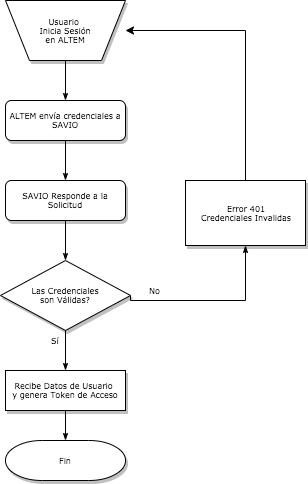
\includegraphics[width=0.6\textwidth]{img/savio_auth.png}
    \caption{Flujo del Middleware de Autenticación con SAVIO }
\end{figure}

\section{Sync. BD Externas}
Se tuvo que desarrollar un sincronizador de datos que recibiera toda la información académica de los estudiantes de la Universidad Tecnológica de Bolívar, por medio de una base de datos proveída por esta entidad la cuál también es de tipo SQL, pero con un vendor diferente (Oracle).

Se utilizó la herramienta SQLines Data para hacer posible migración de datos entre BANNER y ALTEM. 

Este sincronizador obedece los siguientes pasos:

\begin{itemize}
    \item Validar conexión a ambas bases de datos.
    \item Validar existencia de bases de datos en la fuente de datos (BANNER Oracle).
    \item Validar permisos de lectura en las tablas a leer en la fuente de datos.
    \item Truncar las tablas necesarias en la base de datos Destino (ALTEM MySQL).
    \item Realizar la conversión de tipos de datos y espacio para cada una de las columnas de las tablas que se desean migrar
    \item Realizar la copia y conversión de datos de cada una de las filas a transferir
    \item Generar un reporte de la copia de los datos.
\end{itemize}

\begin{figure}[H]
    \centering
    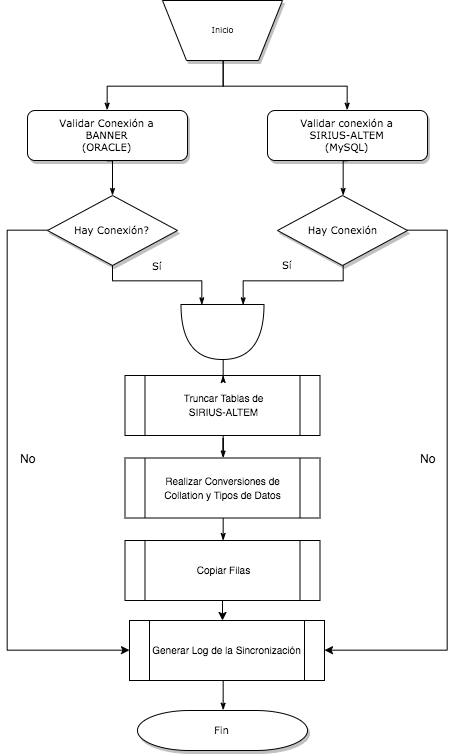
\includegraphics[width=0.6\textwidth]{img/db_sync.png}
    \caption{Flujo de acciones del sincronizador BANNER-ALTEM }
\end{figure}


Este sincronizador se ejecuta semanalmente con el fin de mantener los datos académicos de los estudiantes al día con BANNER.